\chapter{Równoległą implementacja algorytmu ewolucyjnego}
\thispagestyle{chapterBeginStyle}

\section{Użyte technologie}
Do implementacji algorytmu zastosowano język Julia\cite{JULIA-PUB} w wersji 1.3. Julia jest stosunkowo nowym językiem programowania. Został zaprojektowany 
z myślą o zastosowaniach w obliczeniach numerycznych i analizie danych. Łączy on w sobie zalety języków niskopoziomowych i wysokopoziomowych takie jak szybkość 
i czytelność kodu. Testy pokazują, że program napisany w Julii może być równie szybki, jak odpowiadający mu program napisany w C\cite{JULIA-PERFORMANCE}. 
Dodatkową zaletą jest możliwość bezpośredniego wywoływania bibliotek napisanych w C, Fortranie i kilku innych językach popularnych w dziedzinie 
obliczeń numerycznych bezpośrednio z Julii.

Ostatnie aktualizacje w znaczącym stopniu rozwinęły wsparcie języka dla obliczeń równoległych i rozproszonych. W tym momencie Julia oferuje wsparcie dla 
równoległości na poziomie wątków jak i procesów, co dodatkowo wpłynęło na wybór tego właśnie języka. Posiada własny protokół komunikacji między procesami, jednak 
istnieje również biblioteka implementująca najbardziej powszechny protokół MPI.

Julia jest językiem kompilowanym. Używa kompilatora JIT(just-in-time), który kompiluje program tuż przed jego wykonaniem, dzięki czemu jest szybsza 
niż języki interpretowane. Należy pamiętać o tym, że nie każdy program napisany w Julii będzie szybki. Wszystko zależy od jakości dostarczonego kodu.
Głównym czynnikiem, który wpływa na szybkość są typy. Julia jest językiem dynamicznie typowanym, jednak podczas kompilacji tworzone są warianty tej samej 
funkcji dla różnych typów(o ile to możliwe). Pozwala to pominąć kontrolę typów podczas wykonywania kodu i tym samym znacząco przyspieszyć jego działanie.
Dlatego pisząc kod w julii powinniśmy pamiętać o tym, żeby unikać miejsc, w których kompilator będzie zmuszony do konwersji zmiennych do konkretnego typu. 
Aby identyfikować tego typu miejsca możemy używać dostarczonych w bibliotece standardowej narzędzi, które pomagają analizować nasz kod. 
Warte wymienienia są tutaj:
\begin{itemize}
    \item pakiet $Profile$, który zbiera informacje o czasie wywołania kolejnych fragmentów kodu, dzięki czemu w łatwy sposób 
    możemy zidentyfikować fragmenty do dalszej optymalizacji. Pozwala on też śledzić liczbę ilość pamięci alokowanej przez konkretne fragmenty 
    kodu, co również w wielu przypadkach może okazać się przydatną informacją.
    \item makro $@code\_warntype$, które zwraca strukturę AST(abstract syntax tree) dla wykonywanego kodu, dzięki czemu możemy zobaczyć możliwe typy dla wszystkich zmiennych. 
    Dodatkowo miejsca w których kompilator nie jest w stanie jednoznacznie określić typu danej zmiennej jest zaznaczony na czerwono.
\end{itemize}

Julia udostępnia też środowisko uruchomieniowe $REPL$(read-eval-print loop), dzięki któremu możemy w bardzo łatwy sposób testować napisany kod. 
Dzięki dostępnym bibliotekom takim jak $Debugger.jl$ oraz $Rebugger.jl$ możemy w razie potrzeby debugować napisany kod z poziomu $REPL$ co 
znacznie przyspiesza znajdowanie błędów.


\section{Reprezentacja chromosomu}
W opisywanej implementacji jako reprezentacje rozwiązania przyjęto macierz:
$$V = (v_{ij}) \text{, gdzie } 1 \le i \le length(supply) \land 1 \le j \le length(demand)$$

Rozwiązanie jest zakodowane w taki sposób, że komórka macierzy o indeksie $[i, j]$ określa ilość transportowanego towaru 
między $i$-tym punketm nadania i $j$-tym punktem odbioru. Jest to jedna z najbardziej naturalnych reprezentacji rozwiązania 
dla zadania transportowego.

\begin{table}[h!]
    \begin{center}
        \begin{tabular}{c|ccccc}
            i\textbackslash{j} & 10.0 & 7.0 & 5.0 & 13.0 & 12.0 \\ 
            \hline
            12.0 & 0.0 & 7.0 & 5.0 & 0.0 & 0.0 \\
            10.0 & 5.0 & 0.0 & 0.0 & 0.0 & 5.0 \\
            3.0 & 3.0 & 0.0 & 0.0 & 0.0 & 0.0 \\
            10.0 & 0.0 & 0.0 & 0.0 & 3.0 & 7.0 \\
            12.0 & 2.0 & 0.0 & 0.0 & 10.0 & 0.0 \\
        \end{tabular}
    \end{center}
    \caption{Przykładowe rozwiązanie(pierwszy wiersz - wektor punktów odbioru, pierwsza kolumna - wektor punktów nadania).}
\end{table}

Aby ograniczenia zadania zostały zachowane macierz rozwiązania musi spełniać następujące warunki:
$$\sum_{j=1}^{m} v_{ij} = supply[i], \text{ dla } i = 1, 2, \dots, n \text{, gdzie } n = length(supply)$$
$$\sum_{i=1}^{n} v_{ij} = demand[j], \text{ dla } j = 1, 2, \dots, m \text{, gdzie } m = length(demand)$$
$$v_{ij} \ge 0, \text{ dla } i = 1, 2, \dots, n \text{ i } j = 1, 2, \dots, m$$


\section{Inicjalizacja chromosomu}
Projektując procedurę inicjalizacji rozwiązania musimy pamiętać o tym, żeby generowane rozwiązania spełniały ograniczenia przedstawione 
w poprzedniej sekcji oraz obejmowały jak największą część przestrzeni wszystkich rozwiązań. Zaproponowana procedura przyjmuje jako argumenty 
wektory popytu i podaży. Iterując po kolejnych, losowych komórkach macierzy przypisujemy im wartość $val = min(supply[i], demand[j])$, gdzie 
$i, j$ są indeksami wylosowanej komórki macierzy, a $supply[i]$ oraz $demand[j]$ odpowiadającymi im wartościami w wektorach popytu i podaży. 
Następnie zmniejszamy wartości w wektorach o wpisaną wartość $val$. W ten sposób ograniczenia zadania zostają spełnione. Wygenerowane rozwiązania są 
wierzchołkami sympleksu, opisującego wypukły brzeg przestrzeni dopuszczalnych rozwiązań.

\begin{pseudokod}[H]
    \label{inicjalizacja-1}
    \caption{Procedura inicjalizacji chromosomu}
    \KwData{$supply$ - wektor popytu rozmiaru $n$, $demand$ - wektor podaży rozmiaru $m$}
    \KwResult{$V$ - zainicjalizowana macierz}
    \BlankLine
    $V \gets zeros(n, m)$\tcc*[r]{generujemy macierz zerową rozmiaru $n \times m$}
    $indices \gets$ lista wszystkich indeksów macierzy $V$ w losowej kolejności\;
    \BlankLine
    \For{$(s, d) \in indices$} {
        $val \gets min(demand[d], supply[s])$\;
        $demand[d] \gets demand[d] - val$\;
        $supply[s] \gets supply[s] - val$\;
        $V[s, d] \gets val$\;
    }

    \Return{$V$}
\end{pseudokod}

[TODO: Przykład zastosowania]


\section{Operator krzyżowania}
Operator krzyżowania został zdefiniowany jako kombinacja wypukła dwóch rodziców. W ten sposób w wyniku jednego krzyżowania powstają dwa nowe 
rozwiązania.

\begin{pseudokod}[H]
    \label{krzyżowanie}
    \caption{Operator krzyżowania}
    \KwData{$P_1, P_2$ - rodzice wybrani do krzyżowania}
    \KwResult{$O_1, O_2$ - otrzymane dzieci}
    \BlankLine
    $c_1 \gets rand(0,\dots,1)$\tcc*[r]{losujemy liczbę z przedziału $[0,1]$}
    $c_2 \gets 1.0 - c_1$\;
    $O_1 \gets c_1 * P_1 + c_2 * P_2$\;
    $O_2 \gets c_2 * P_1 + c_1 * P_2$\;
    \Return{$(O_1, O_2)$}\;
\end{pseudokod}

Zdefiniowany tak operator krzyżowania nie narusza ograniczeń zadania, ponieważ przestrzeń rozwiązań jest wypukła. Wynika z tego, że jeśli 
rodzice spełniali ograniczenia, to otrzymane w ten sposób dzieci również muszą spełniać ograniczenia.

[TODO: Przykład zastosowania]

\section{Operator mutacji}
Operator mutacji opiera się na modyfikacji rozwiązania poprzez wybranie z niego podmacierzy i jej ponowną inicjalizacje(patrz \ref{mutacja}). 
Załóżmy, że mamy $n$ punktów nadania i $m$ punktów odbioru. Wybierzmy jako kandydata do mutacji macierz $V = (v_{ij})$, gdzie $1 \le i \le n$ i 
$1 \le j \le m$. Podmacierz $W = w_{ij}$ jest tworzona w następujący sposób:

\begin{itemize}
    \item Losujemy podzbiór $k$ indeksów $\{i_1, \dots, i_k\}$ ze zbioru $\{1, \dots, n\}$ oraz podzbiór $l$ indeksów $\{j_1, \dots, j_l\}$ 
    ze zbioru $\{1, \dots, m\}$, $2 \le k \le n$ i $2 \le l \le m$.
    \item Tworzymy podmacierz $W$ składającą się z takich elementów macierzy $V$, które zostały wylosowane, tzn. element $v_{ij} \in V$ 
    zostaje włączony do podmacierzy $W$ tylko jeśli $i \in \{i_1, \dots, i_n\}$ oraz $j \in \{j_1, \dots, j_l\}$.
\end{itemize}

Dla stworzonej macierzy $W$ tworzymy nowe wektory $demand_W$ i $supply_W$ w następujący sposób:
$$supply_W[i] = \sum_{j \in \{j_1, \dots, j_l\}} v_{ij}, \text{ dla } 1 \le i \le k$$
$$demand_W[j] = \sum_{i \in \{i_1, \dots, i_k\}} v_{ij}, \text{ dla } 1 \le j \le l$$

Następnie na nowo inicjalizujemy podmacierz $W$ macierzy $V$ używając stworzonych wektorów $demand_W$ oraz $supply_W$ do określenia popytu i podaży 
w wybranych punktach nadania i odbioru. Po zakończeniu inicjalizacji przepisujemy wartości z podmacierzy $W$ z powrotem w odpowiadające miejsca 
macierzy $V$.

\begin{pseudokod}[H]
    \label{mutacja}
    \caption{Operator mutacji}
    \KwData{$V$ - osobnik wybrany do mutacji wielkości $n \times m$, $k, l$ - wielkość podmacierzy}
    \KwResult{$V$ - osobnik po mutacji}
    \BlankLine
    $supply\_idx \gets$ wylosuj podzbiór długości $k$ ze zbioru $\{1, \dots, n\}$\;
    $demand\_idx \gets$ wylosuj podzbiór długości $l$ ze zbioru $\{1, \dots, m\}$\;
    $W \gets zeros(k, l)$\tcc*[r]{generujemy macierz zerową rozmiaru $k \times l$}
    \BlankLine
    \For{$i \in \{1, \dots, k\}$} {
        \For{$j \in \{1, \dots, l\}$} {
            $W[i, j] \gets V[demand\_idx[j], supply\_idx[i]]$\;
        }
    }
    \BlankLine
    $supply\_vec \gets zeros(k)$\tcc*[r]{generujemy wektor zerowy długości k}
    $demand\_vec \gets zeros(l)$\tcc*[r]{generujemy wektor zerowy długości l}
    \BlankLine
    \For{$i \in supply\_idx$} {
        $supply\_vec[i] \gets \sum_{j \in demand\_idx} V[i, j]$\;
    }
    \BlankLine
    \For{$j \in demand\_idx$} {
        $demand\_vec[j] \gets \sum_{i \in supply\_idx} V[i, j]$\;
    }
    \BlankLine
    $W \gets inicjalizacja(W, demand\_vec, supply\_vec)$\;
    \BlankLine
    \For{$i \in \{1, \dots, k\}$} {
        \For{$j \in \{1, \dots, l\}$} {
            $V[demand\_idx[j], supply\_idx[i]] \gets W[i, j]$\;
        }
    }
    
    \Return{$V$}
\end{pseudokod}

Zdefiniowano dwa operatory mutacji. Różnią się one jedynie procedurą inicjalizacji. W pierwszym używamy tej samej procedury, którą inicjalizujemy 
nowe chromosomy podczas generowania populacji początkowej(patrz \ref{inicjalizacja-1}). Druga jest modyfikacją tej procedury. Modyfikacja polega na tym, że zamiast wybierać 
jako wartość pola $val = min(demand[j], supply[i])$ wybieramy liczbę z zakresu $[0, val]$. Zmiana ta powoduje, że otrzymana macierz może naruszać 
ograniczenia zadania, dlatego po wstępnym wyznaczeniu wartości naprawiamy rozwiązanie poprzez zrobienie wymaganych dodawań w taki sposób, żeby 
rozwiązanie spełniało ograniczenia. 

Poniżej przedstawiono schemat zmodyfikowanej procedury inicjalizacji w postaci pseudokodu.

\begin{pseudokod}[H]
    \label{inicjalizacja-2}
    \caption{Zmodyfikowana procedura inicjalizacji}
    \KwData{$supply$ - wektor podaży rozmiaru $n$, $demand$ - wektor popytu rozmiaru $m$}
    \KwResult{$V$ - zainicjalizowana macierz}
    \BlankLine
    $V \gets zeros(n, m)$\tcc*[r]{generujemy macierz zerową rozmiaru $n \times m$}
    $indices \gets$ lista wszystkich indeksów macierzy $V$ w losowej kolejności\;
    \BlankLine
    \For{$(s, d) \in indices$} {
        $val \gets$ wartość z przedziału $[0, min(demand[d], supply[s])]$\;
        $demand[d] \gets demand[d] - val$\;
        $supply[s] \gets supply[s] - val$\;
        $V[s, d] \gets val$\;
    }
    \BlankLine
    \For{$(s, d) \in indices$} {
        $val \gets min(demand[d], supply[s])$\;
        $demand[d] \gets demand[d] - val$\;
        $supply[s] \gets supply[s] - val$\;
        $V[s, d] \gets V[s, d] + val$\;
    }

    \Return{$V$}
\end{pseudokod}

[TODO: Przykład zastosowania]

\section{Funkcje oceny}
W przypadku omawianego problemu funkcja oceny jest równoważna funkcji celu dla zadania transportowego. Powinna więc mieć postać:
$$\sum_{i=1}^{n}\sum_{j=1}^{m} f(v_{ij})$$, 
gdzie $f(v_{ij})$ jest dowolną funkcją przyjmującą jako argument ilość towaru transportowanego między punktami $i$ oraz $j$.

[TODO: Przykłady funkcji oceny użyte w części eksperymentalnej + wykresy]

\section{Metoda selekcji}
W algorytmie zastosowano standardową metodę selekcji - metodę koła ruletki. W tej metodzie lepiej przystosowane osobniki mają odpowiednio większe 
szanse na to, że zostaną wybrane do puli rodziców dla następnej generacji. Polega ona na tym, że dla każdego osobnika z populacji 
przyporzątkowujemy odpowiednio duży wycinek koła. Wielkość wycinka zależy od wartości funkcji przystosowania, jaką osiągnął dany chromosom. 
Następnie losujemy kołem tyle razy, ile rodziców chcemy otrzymać. Metoda ta pozwala na to, że jeden osobnik zostanie wybrany na rodzica kilkukrotnie.

Bardziej formalnie procedura została przedstawiona na poniższym pseudokodzie.

\begin{pseudokod}[H]
    \label{selekcja}
    \caption{Procedura selekcji}
    \KwData{$population$ - populacja chromosomów, $n$ - ilość rodziców do wybrania}
    \KwResult{$parents$ - wektor wybranych rodziców}
    \BlankLine
    $parents \gets$ stwórz pusty wektor długości n\;
    $k \gets length(population)$\;
    $wheel \gets zeros(k)$\tcc*[r]{Generujemy wektor zerowy długości $n$}
    \BlankLine
    $total \gets \sum_{i=1}^{k} population[i].cost$\;
    $wheel[1] \gets population[1].cost / total$\;
    \For{$i \in 2,\dots, k$} {
        $wheel[i] \gets population[i].cost / total + wheel[i-1]$\;
    }
    \BlankLine
    \For{$i \in 1,\dots, n$} {
        $num \gets rand(0,\dots, 1)$\tcc*[r]{losujemy wycinek koła}
        $selectedIdx \gets$ wybierz pierwszy taki $x$, że $x \le num$\;
        $parents[i] \gets population[selectedIdx]$\;
    }

    \Return{$parents$}
\end{pseudokod}

% Na początku obliczana jest suma kumulatywna dla całego pokolenia. Następnie 
% otrzymane wartości skalujemy tak, aby znajdowały się w przedziale $[0, 1]$. W ten sposób przedział $[0, 1]$ zostaje podzielony na mniejsze, które 
% odpowiadają pojedynczym osobnikom z populacji. Następnie generujemy losową liczbę z tego przedziału. Do zbioru rodziców dodawany jest osobnik, 
% w którego przedziale znajduje się wylosowana liczba. Warto zauważyć że tak zaprojektowana selekcja pozwala na to, że jeden osobnik zostanie wybany 
% kilkukrotnie na rodzica.

[TODO: obrazek ilustrujący algorytm]

\section{Wersja równoległa}
Algorytm może działać w dwóch trybach:
\begin{itemize}
    \item Klasycznym
    \item Wyspowym
\end{itemize}

Na początku procedura inicjalizacji generuje losową populacje o określonej liczbie osobników i oblicza wartość funkcji oceny dla każdego z nich. 
Następnie przechodzimy do głównej pętli algorytmu, która kończy się w momencie kiedy populacja osiągnie maksymalną ilość generacji. 
Każdy z trybów różni się przebiegiem procedury \textit{nextGeneration}(patrz \ref{alg_main_img}), która tworzy nową generacje osobników.

\begin{figure}[H]
    \centering        
    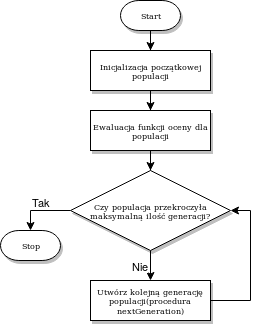
\includegraphics[width=0.4\textwidth]{img/alg_main.png}
    \caption{Przebieg zaimplementowanego algorytmu ewolucyjnego}
    \label{alg_main_img}
\end{figure}

Model klasyczny nie różni się wiele od standardowego algorytmu ewolucyjnego. Mamy tutaj jedną populacje, która ewoluuje przez 
określoną na starcie liczbę pokoleń. Wszystkie dostępne parametry algorytmu oraz ich dopuszczalne wartości opisane są w dalczej części pracy, 
w sekcji \textit{Pliki konfiguracyjne}.

W modelu klasycznym zrównoleglenie odbywa się na poziomie pojedynczej iteracji(patrz \ref{next_gen_klasyczny_img}). 
Ewolucję populacji możemy podzielić tutaj na dwie części:
\begin{itemize}
    \item \textbf{Krzyżowanie} - w tej części między wątki rozdzielani są rodzice wybrani do krzyżowania. Następnie każdy z wątków generuje swoją część 
    dzieci oraz z określonym prawdopodobieństwem stostuje na nich operator mutacji i ostatecznie oblicza dla nich wartość funkcji oceny. 
    Dzieci są dodawane do kolejnej populacji.
    \item \textbf{Dopełnienie populacji} - w tej części do kolejnej populacji przepisywana jest część najlepszych rozwiązań oraz losowo wybranych osobników 
    z poprzedniej populacji. Następnie te dodane osobniki są poddawane mutacji i obliczana jest dla nich funkcja oceny.
\end{itemize}

\begin{figure}[H]
    \centering        
    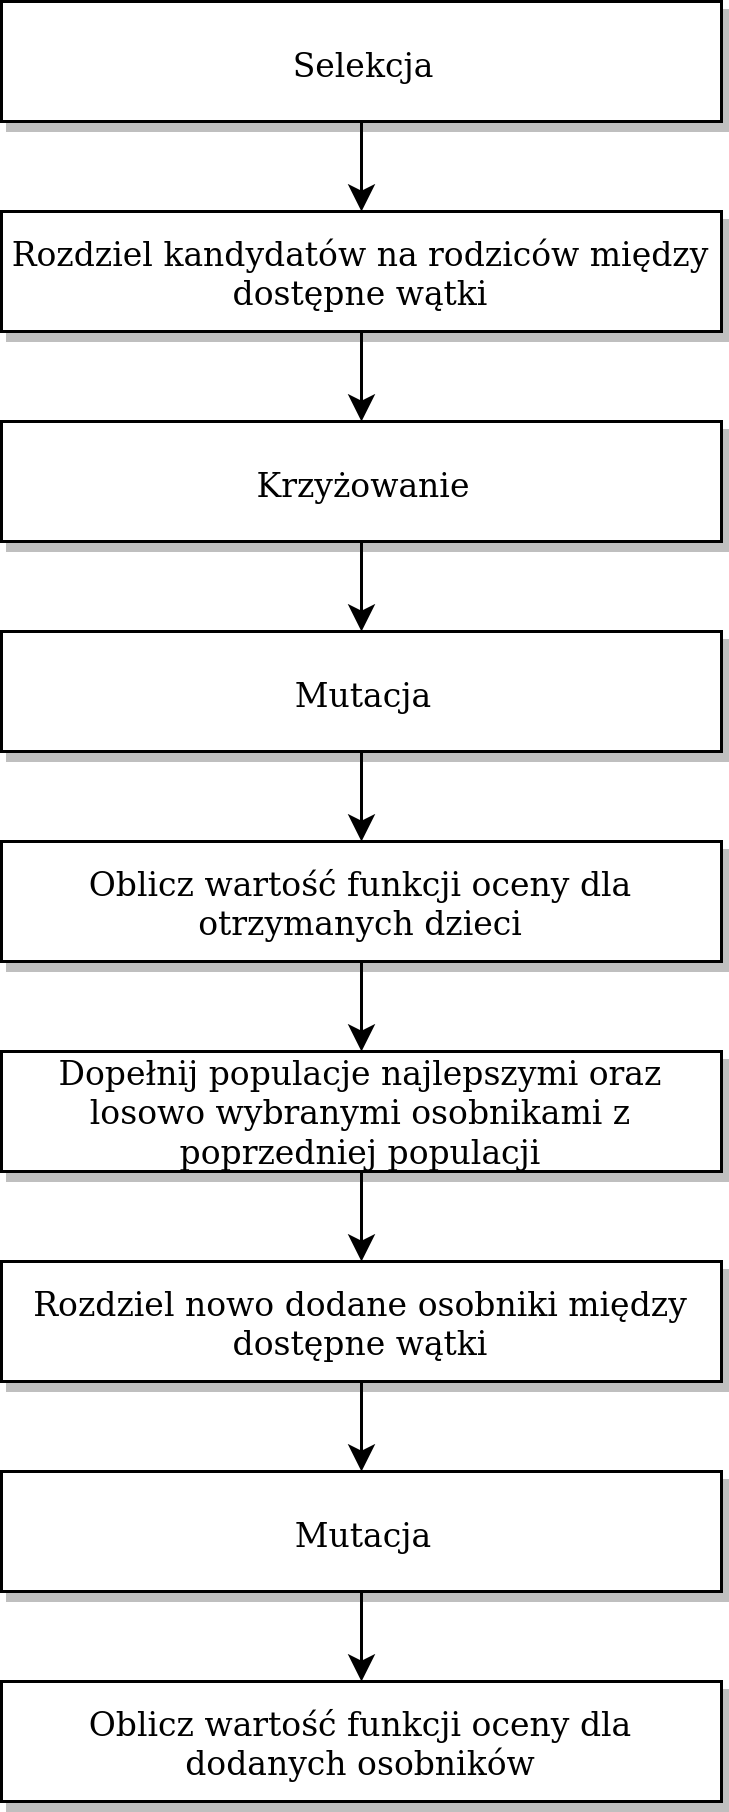
\includegraphics[width=0.2\textwidth]{img/next_gen_klasyczny.png}
    \caption{Przebieg procedury nextGeneration dla modelu klasycznego}
    \label{next_gen_klasyczny_img}
\end{figure}

Model wyspowy różni się od klasycznego podejścia tym, że całkowita populacja jest tutaj rozdzielana na kilka mniejszych. Następnie każda z 
populacji częściowych ewoluuje niezależnie od innych przez określoną liczbę pokoleń. Po zakończeniu tego procesu wszystkie częściowe populacje 
są na nowo łączone w jedną. Następnie najlepsze rozwiązywanie jest zapisywane, a populacja zostaje na nowo podzielona na kilka mniejszych i 
cały proces się powtarza, do momentu w którym ilość generacji przekroczy określoną na początku liczbę. Na końcu najlepsze znalezione rozwiązanie 
jest zwracane.

W tym modelu zrównoleglenie obliczeń polega na tym, że przy każdym podziale populacji jeden wątek zarządza pojedynczą częścią populacji(patrz \ref{next_gen_wyspowy_img}).
Model ten skaluje się lepiej niż model klasyczny ze względu na to że podzadania przydzielane wątkom są większe. Minusem jest tutaj to, że populacja 
musi być odpowiednio duża, żeby jej podział na mniejsze części się sprawdził.

\begin{figure}[H]
    \centering        
    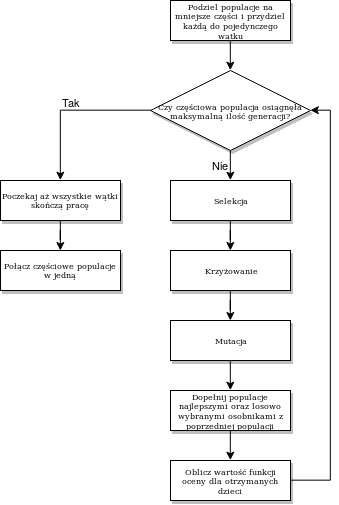
\includegraphics[width=0.5\textwidth]{img/next_gen_wyspowy.png}
    \caption{Przebieg procedury nextGeneration dla modelu wyspowego}
    \label{next_gen_wyspowy_img}
\end{figure}

W tym momencie każda z częściowych populacji w modelu wyspowym posiada takie same parametry. [...]

\section{Pliki konfiguracyjne}
Dodatkowo do algorytmu został dodany moduł obsługi plików konfiguracyjnych. Używają one formatu JSON. Moduł pozwala na zapisywanie i wczytywanie 
całej konfiguracji algorytmu, w skład której wchodzą wektory popytu i podaży, macierz kosztu, oraz wszystkie parametry programu.
Definicja poszczególnych parametrów:

\begin{itemize}
    \item $populationSize$ - rozmiar całkowitej populacji. Powinien być dodatnią liczbą całkowitą.
    \item $eliteProc$ - ułamek najlepszych rozwiązań, które zostają przepisane do następnego pokolenia. 
    Wartość powinna znajdować się w przedziale $[0, 1]$. Testy pokazują, że najlepsze rozwiązania są generowane dla wartości parametru w przedziale
    $[0.1, 0.3]$.
    \item $mutationProb$ - prawdopodobieństwo mutacji. Przyjmuje wartość z zakresu $[0, 1]$. Warto pamiętać o tym, że zalecane prawdopodobieństwo 
    mutacji nie powinno przekraczać kilkanastu procent.
    \item $mutationRate$ - wielkość mutacji, określa stosunek rozmiaru podmacierzy, wybieranej do ponownej inicjalizacji podczas mutacji, 
    do macierzy rozwiązania. Przyjmuje wartości z zakresu $[0, 1]$. Tak jak w przypadku prawdopodobieństwa mutacji, jej wielkość nie powinna 
    przekraczać kilkunastu procent, ponieważ zbyt duża mutacja może niszczyć znalezione rozwiązania.
    \item $crossoverProb$ - prawdopodobieństwo krzyżowania. Przyjmuje wartości z przedziału $[0, 1]$. Zaleca się ustawialnie wartości z przedziału 
    $[0.5, 0.9]$. Należy pamiętać o tym, że suma parametrów eliteProc i crossoverProb nie może być większa niż $1$.
    \item mode - tryb w jakim ma działać algorytm. Przyjmuje wartości $regular$(w przypadku wyboru klasycznego modelu) lub $island$(w przypadku 
    modelu wyspowego).
    \item $numberOfSeparateGenerations$ - liczba naturalna określająca ilość iteracji jakie wykona algorytm pomiędzy rozdzieleniem populacji na 
    mniejsze części, a ponownym jej scaleniem. Dla wyboru modelu klasycznego należy ustawić wartość parametru na $1$.
\end{itemize}

Dodatkowo w pliku konfiguracyjnym określamy wektor popytu, podaży i macierz kosztów:

\begin{itemize}
    \item $demand$ - wektor popytu. Przyjmuje jako wartość listę elementów, które składają się z dwóch pól - $i$, które określa indeks wektora i 
    $val$, które określa wartosć wektora w miejscu $i$ - $demand[i] = val$.
    \item $supply$ - wektor podaży. Przyjmuje jako wartość listę elementów, o polach takich samych jak w przypadku wektora popytu. Pojedynczy element 
    opisuje pole wektora $supply[i] = val$.
    \item $costMatrix$ - macierz kosztu, która może być wykorzystywana w funkcji celu. Przyjmuje jako wartość listę elementów, które składają się 
    z trzech pól: $s$ - określa indeks odpowiadający indeksowi wektora podaży, $d$ - określa indeks odpowiadający indeksowi wektora popytu, oraz 
    $val$ - określa wartość macierzy w polu o podanych indeksach $costMatrix[d, s] = val$.
\end{itemize}

Przykładowy plik konfiguracyjny:

\begin{lstlisting}[language=json, firstnumber=1, frame=single]
{
    "populationSize": 100,
    "eliteProc": 0.3,
    "mutationProb": 0.1,
    "mutationRate": 0.05,
    "crossoverProb": 0.2,
    "mode": "regular",
    "numberOfSeparateGenerations": 1,
    "demand": [
        {
            "val": 1.0,
            "i": 1
        },
        {
            "val": 10.0,
            "i": 2
        }
    ],
    "supply": [
        {
            "val": 1.0,
            "i": 1
        },
        {
            "val": 5.0,
            "i": 2
        },
        {
            "val": 5.0,
            "i": 3
        }
    ],
    "costMatrix": [
        {
            "val": 1.0,
            "s": 1,
            "d": 1
        },
        {
            "val": 2.0,
            "s": 2,
            "d": 1
        },
        {
            "val": 3.0,
            "s": 3,
            "d": 1
        },
        {
            "val": 10.0,
            "s": 1,
            "d": 2
        },
        {
            "val": 20.0,
            "s": 2,
            "d": 2
        },
        {
            "val": 30.0,
            "s": 3,
            "d": 2
        }
    ]
}
\end{lstlisting}